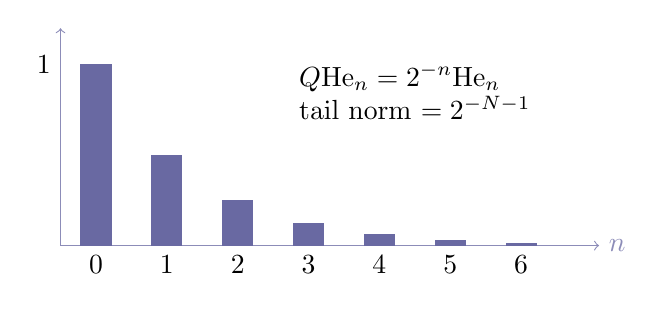
\begin{tikzpicture}[x=.9cm,y=2.3cm]
\draw[->,MidnightBlue!50] (-.5,0)--(7.1,0) node[right] {$n$};
\draw[->,MidnightBlue!50] (-.5,0)--(-.5,1.2);
\foreach \n in {0,...,6}{
\fill[MidnightBlue!65] (\n-.22,0) rectangle (\n+.22,{pow(.5,\n)});
\node[below] at (\n,0) {$\n$};
}
\node[left] at (-.5,1) {$1$};
\node[align=left] at (4.5,.85) {$Q\mathrm{He}_n=2^{-n}\mathrm{He}_n$\\tail norm $=2^{-N-1}$};
\end{tikzpicture}
